\section{Implementation Issues}\label{sec-imp}

In this section, we discuss the issue of implementing the protocol proposed
in the previous section. One issue is that the Internet currently does not
support a protocol without sender information. We propose two ways of
implementing our One-Way protocol: using trusted gateways, and on top of
UDP transport layer protocol~\cite{RFC768}.

\subsection{Trust Gateway}

In trust gateway method, we envision implementing our protocol in hardware
with a wireless access point that understands our One-Way protocol.
In method the network topology is divided into two parts: a private
network that understands the One-Way protocol and the rest of the world that
only understand the IP protocol as shown in Figure~\ref{fig:gateway}. The
gateway acts as normal wireless access point and multiplex traffic for the
peers inside the private network.

\begin{figure}[h]
\begin{center}
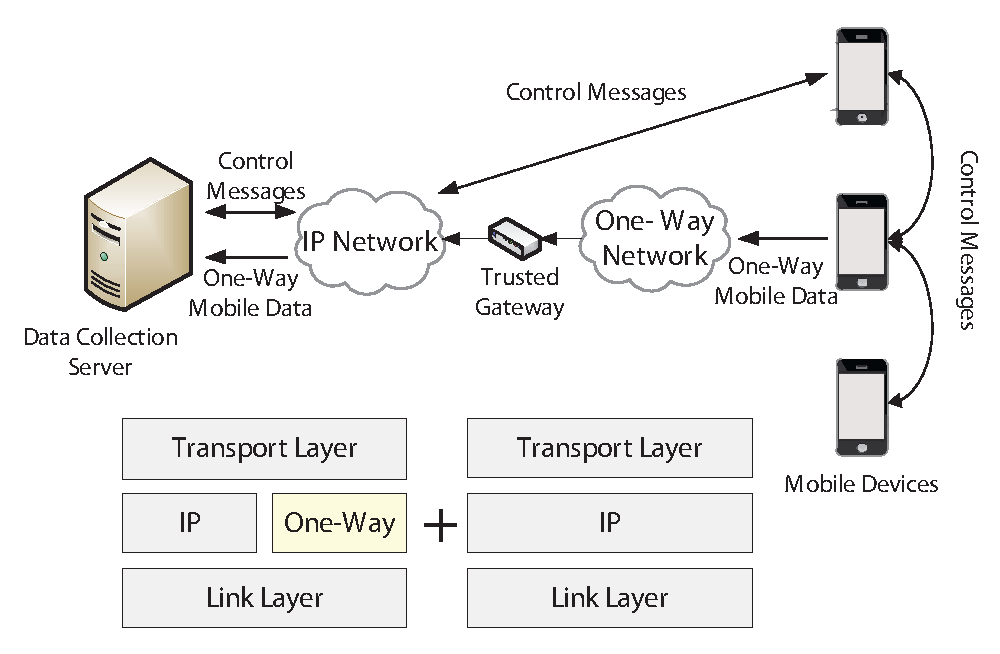
\includegraphics[width=3.4in]{one-way-gateway.eps}
\caption{\small \sl Trusted Gateway.\label{fig:gateway}}
\end{center}
\end{figure}

%\begin{figure}[h]
%\begin{center}
%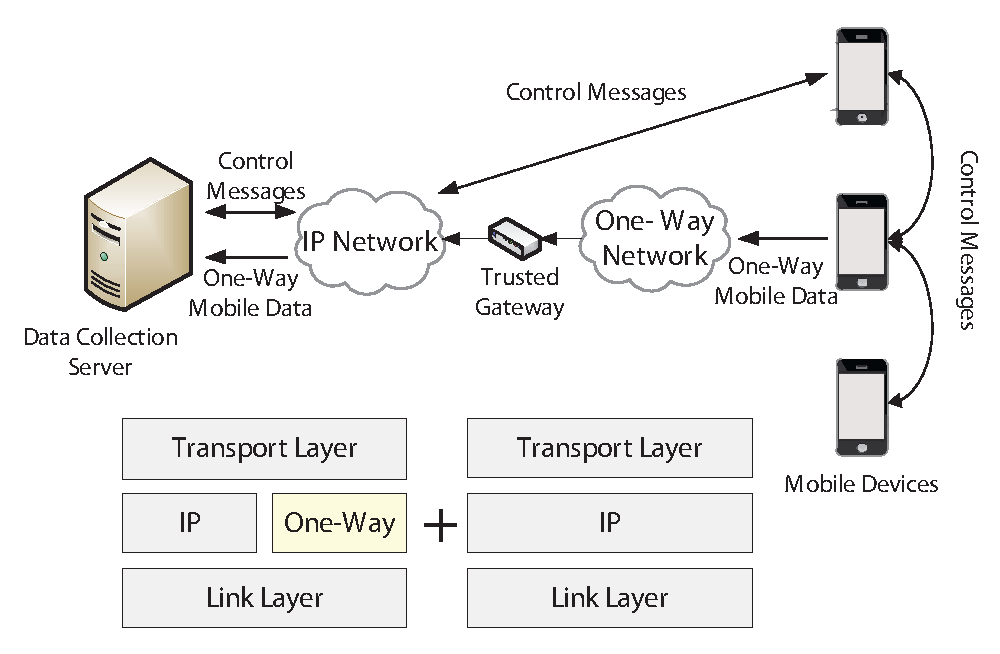
\includegraphics[width=3in]{one-way-gateway.eps}
%\caption{\small \sl Stack for Trusted Gateway.\label{fig:gateway_b}}
%\end{center}
%\end{figure}

Since the control message protocol does not have the issue of concealing
the sender routing address, the validation route is construct on the
normal UDP/IP network. When a peer wants to sends a file to a data
collection server, it finds a peers on the traditional IP network that
runs our protocol. Afterwards, the sender construct a connection request
message and sends the message to the peer. The first peer forwards the
request to a second peer and so on until the hop count of the request and
the request is sent to the server.

When sending a payload message, the sender sends the message through the
trusted gateway. Upon receiving a payload message, the gateway performs a
tunneling operation and transforms the message into an UDP packet including
all necessary information for the protocol in the packet, using its own
identity in the packet header, then forwards the packet into the IP network.
Since the gateway uses it own
IP address as the address of the packets, it shields the identity of the mobile
clients. A reason for this tunneling approach is that some Internet service
providers (ISP) will block packets without valid source host address.
Figure~\ref{fig:gateway_b}
depicts the networking stack configuration of this approach.

Opponents of this approach could argument that attacker can still
trace the mobile clients to a
specific subnet where the gateway device resides. We argue that since most of
the clients are highly mobile, and with a number of access points in one
geographic region, the identity of the mobile devices can be protected with high
confidence.

\subsection{Over User Datagram Protocol}
If a subnet allows packet with anonymous sender IP address (such as the
broadcast address) to be forwarded through the network, then we can build
our protocol on top of existing network protocol.
In this approach, we completely do away with a new access point by building
the One-Way protocol as an application layer protocol on top of User Datagram
Protocol (UDP) and use existing network hardware and infrastructure. This
method is illustrated in Figure~\ref{fig:imp-udp}.

\begin{figure}[h]
\begin{center}
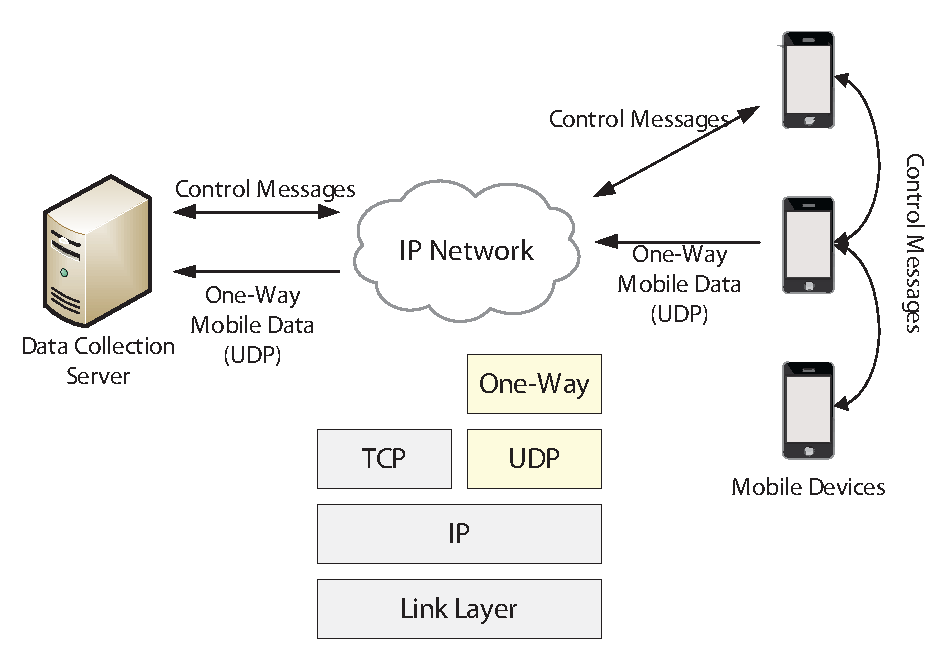
\includegraphics[width=3.4in]{one-way-udp.eps}
\caption{\small \sl One-Way over UDP.\label{fig:imp-udp}}
\end{center}
\end{figure}

The steps for making a connection request is the same for the trusted
gateway approach, but payload transmission is slightly different.
During payload transmission, instead of letting a gateway to replace the
identity of the packets, the sender uses the broadcast IP address
(255.255.255.255) in the sender address field of the packet. This denote
that the sender is anonymous and the server should treat the data transmission
using anonymous protocol.

Note that the reason we use UDP is that TCP will not work in our approach
because it is connection oriented protocol. With arbitrary IP address field,
TCP will be unable to establish a connection with the handshaking protocol.

%In our experiment, we are able to send IP packets with arbitrary source address into
%the network and receive it on the server. 